\documentclass[12pt]{article}
%%%%%%%%%%%%%%%%%%%%%%%%%%%%%%
%Force pdflatex processing even with "$ latex" (required by arXiv)
\pdfoutput=1
%%%%%%%%%%%%%%%%%%%%%%%%%%%%%
\usepackage[top=3cm, bottom=3cm, left=2cm, right=2cm]{geometry}
\usepackage[usenames,dvipsnames,svgnames]{xcolor}
\definecolor{darkblue}{rgb}{0.0,0.1,0.3} % dark blue
\definecolor{darkgreen}{rgb}{0,0.65,0}
\definecolor{dblue4}{rgb}{0.06,0.31,0.55} % DodgerBlue4
\definecolor{nicered}{rgb}{0.7,0.1,0.1}
\definecolor{nicegreen}{rgb}{0.1,0.5,0.1}

\usepackage[numbers,sort&compress]{natbib}
%\usepackage{cite}

\usepackage[utf8]{inputenc}
\usepackage{textcomp}
\usepackage{amsmath,amssymb,amsfonts,amsthm}
%\usepackage{siunitx} 
\usepackage{tabularx}
\usepackage{multirow}
\usepackage{dsfont}
\newcolumntype{Y}{>{\centering\arraybackslash}X}

\usepackage{xcolor}
\usepackage[colorlinks=true,citecolor= nicegreen,linkcolor=nicered]{hyperref}

\usepackage{verbatim} 
\usepackage{graphicx}
\graphicspath{{figures/}}
\usepackage{cancel}

\usepackage[colorinlistoftodos]{todonotes}

\usepackage{comment}
\includecomment{details}
\specialcomment{details}
{\begingroup}{\endgroup}
\excludecomment{details}
%\PreviewEnvironment{details}
%%%%%%
%Custom definitions
\usepackage{tikz}
\newcommand{\ReportNumbers}[1]{%
\begin{tikzpicture}[overlay, remember picture]
\path (current page.north east) ++(-1,-1) node[below left] {#1};
\end{tikzpicture}
}
%%%%%%%%%%%%%%%TITLE PAGE

\title{Dirac neutrino mass generation from Majorana messenger}

\author{First Author\footnote{\href{mailto:first@author}{first@author}},
Second Author\footnote{\href{mailto:second@author}{second@author}}\\
\textit{\small  First Institute}\\
[4mm]
Third Author\footnote{\href{mailto:third@author }{third@author}}\\
\textit{\small Second Institute}
}
\date{\small Month NN, YYYY}
\begin{document}
\maketitle
\ReportNumbers{XXX-XXX}

\begin{abstract}    
We propose a model for one-loop Dirac neutrino masses with Majorana mediators which can be dark matter candidates if they are the lightest states circulating the loop. This model is restricted by  neutrino physics,  lepton flavor violation and cosmological constrains, including  
the effective number light neutrinos $N_{\text{eff}}$. Here we find that $M_{Z^{\prime}}/g^{\prime} \gtrsim 60\ \text{TeV}$ in order to satisfy the conditions of $N_{\text{eff}}$..
\end{abstract}

\section{Introduction}
\label{sec:intro}
%Dirac or Majorana
The interpretation of neutrino experimental data in terms of neutrino
oscillations is compatible with both Majorana or Dirac neutrino masses
\cite{Tanabashi:2018oca}. The former possibility has received the most
attention but, given the lack of signals in neutrinoless double beta
decay experiments
\cite{KamLAND-Zen:2016pfg,Agostini:2018tnm,Aalseth:2017btx,Alduino:2017ehq,Albert:2017owj,Arnold:2016bed},
the latter cannot be dismissed.
% Dirac case
If neutrinos are Dirac particles, the Standard Model (SM) particle
content must be extended with right-handed neutrinos,
% with cosmology implications
which can increase the effective number of light neutrinos,
$N_{\text{eff}}$, until 6. Therefore, to be compatible with the
current cosmological restrictions on $N_{\text{eff}}$, the
interactions of the extra right-handed neutrinos with the primordial
plasma must be highly suppressed.

%Smallness of neutrinos for both Dirac and Majorana
On the other hand, to give small masses to at least two Majorana or
Dirac neutrinos, as required to explain the neutrino oscillation
experiments~\cite{Ahmad:2002jz, Fukuda:1998mi},
%focus in seesaw type I
the seesaw mechanism with heavy fermions is usually invoked.
%tree-level case
For the tree-level type-I seesaw we can have either light Majorana
neutrinos with heavy Majorana
mediators~\cite{Minkowski:1977sc,Yanagida:1979as,GellMann:1980vs,Mohapatra:1979ia}
or light Dirac neutrinos with heavy Dirac
mediators~\cite{Roncadelli:1983ty,Roy:1983be,Gu:2007mc,Ma:2014qra}.
%one-loop case
The radiative type-I seesaw includes both~\cite{Ma:2006km}
possibilities~\cite{Farzan:2012sa},
%new possibility in radiative case
but now it is also possible to have light Majorana neutrinos with
heavy Dirac mediators~\cite{Ma:2013yga}.
%New in this work
In this work we want to explore the possibility to build a simple
Dirac radiative type-I seesaw model with heavy Majorana mediators.
%Old idea but first realized here
It is worth noticing that this idea have been already illustrated in
an extension of the minimal supersymmetric standard
model~\cite{Demir:2007dt} but without show any explicit solution.

%Features of the new propossed solution
In general, solutions for light Dirac neutrino masses require a
continuous symmetry to guarantee their Diracness. This symmetry is
usually identified as the $\operatorname{U}(1)_{B-L}$.  Additionally,
ad-hoc discrete symmetries are invoked to forbid tree level Dirac or
Majorana mass terms for the light right-handed
neutrinos~\cite{Roncadelli:1983ty,Han:2018zcn,Wang:2017mcy}. 
%tree-level without adhoc symmetries
However, tree-level Dirac type-I seesaw with proper choices for the
$\operatorname{U}(1)_{B-L}$ charges have been shown to be consistent
without require any extra ad-hoc discrete symmetries~\cite{Ma:2014qra}.
%one-loop 
In recent works, it has been shown that even for one-loop Dirac
neutrino masses, it is possible to have $\operatorname{U}(1)_{B-L}$ as
the only extra symmetry beyond the SM~\cite{Calle:2018ovc,Bonilla:2018ynb,Saad:2019bqf}\footnote{
%extra-loops
  For extensions with only extra scalars, minimal solutions have been found with two and three loops~\cite{Saad:2019bqf}}.
%conexion with dark matter
As a bonus in this case, the new scalars and fermions circulating the
loop can be dark matter candidates with the stability of the lightest
of them guaranteed by the very same continuous symmetry.
% remark
We focus here in solutions for the radiative Dirac type-I seesaw with
Majorana mediators, which have only an extra symmetry responsible for the
Diracness of the light neutrinos, the absence of any tree-level
mass, and the existence of a dark sector constituted by the
particles circulating the loop.

%conexion with DM
In fact, another evidence that the SM is not a complete theory is the
missing matter content of the universe, which is known as dark matter
(DM).
% DM as particle
The main proposals that explain DM as a particle are given in
Ref.~\cite{Bertone:2004pz}.
% too many possibilities
Without evidence of DM as a particle there is not a clear path to pin
out the DM properties nor the possible heavier companions of some
extended sector. 
% connect with other phenomena
Linking the dark sector to other specific phenomenology allows to
reduce the arbitrariness in the model building.
% loop
In our construction, the dark sector is related to the heavy sector
responsible of the lightness of the neutrinos and the same symmetry
which guarantees the lightness of the Dirac neutrinos is the
responsible of the stability of the lightest dark particle (LDP).
% new particle prediction
Therefore, the number of specific models is quite restricted.

% We will make use of the scotogenic model~\cite{Ma:2006km}. In
% scotogenic model the neutrino masses and the DM have common
% explanation. The neutrino masses are generated by one-loop effects,
% where the candidates for DM are mediators in the loop.
%Conclusion:
In this work we propose a radiative Dirac type-I seesaw, with Majorana
fermions as mediators in the loop. This full set of mediators in the
loop can include a DM candidate.

The rest of the paper is organized as follows. In the next section we present the model and the particle content. In the section~\ref{sec:ScaMassSpect} we study the scalar mass spectrum after spontaneous symmetry breaking. In section~\ref{sec:Neutrinos} We present a mechanism to generate Dirac neutrino masses. In section~\ref{sec:LFV} we show the lepton flavor violation (LFV) experimental  constraints. Finally, in the section~\ref{sec:DM} we present the viable DM candidates.

\section{The model}
\label{sec:Model}
%
\begin{table}[t!]
  \centering
  \begin{tabular}{|c|c|c|c|}
    \hline  
    Fields     & $\operatorname{SU}(2)_L$ & $\operatorname{U}(1)_Y $ & $\operatorname{U}(1)_X$ \\ \hline
    % $H $  & 2  1/2  &  0 \\
    $\eta$  & $\boldsymbol{2}$ & $1/2$  & $1$ \\
    $S$ & $\boldsymbol{1}$ & $0$  & $2$ \\
    $\sigma$ & $\boldsymbol{1}$ & $0$ & $3$ \\
    \hline
    % $Q_{L_{i}}$  & $(2,-1/6)$ & $0$ \\
    % $\overline{u_{R_{i}}}$ & $(1,-2/3)$ & $0$ \\
    % $\overline{d_{R_{i}}}$ & $(1,1/3)$ & $0$ \\
    % \hline
    % $L_i$  & $(2,-1/2)$ & $0$ \\
    % $\overline{e_{R_i}}$ & $(1,1)$ & $0$ \\
    $\nu_{Ri}$ & $\boldsymbol{1}$ & $0$ & $-4$\\
    $\nu_{R3}$ & $\boldsymbol{1}$ & $0$ & $5$\\
    $\psi_{R\alpha}$  & $\boldsymbol{1}$ & 0 & $1$ \\\hline
  \end{tabular}
  \caption{The new scalars and fermions with their respective charges. All the SM fields are neutral under the new $\operatorname{U}(1)_X$ gauge symmetry. }
    \label{tab:partcont}
\end{table}
%
We extend the standard model with a spontaneously broken Abelian gauge symmetry  which guarantees the total lepton number ($L$) conservation. Only the new particles including the light right handed neutrinos are charged under this symmetry. We choose the new particle set such that the following dimension six operator is genuinely realized
\begin{align}
  \label{eq:ld6}
  \mathcal{L}_{6D}=\frac{1}{\Lambda^2} \overline{L_i} H \nu_R S^2\,,
\end{align}
where $S$ is the singlet scalar field which can spontanouely break the $\operatorname{U}(1)_X$ symmetry.

With the aim to illustrate the one-loop Dirac neutrino mass generation
we consider the particle content shown in Table \ref{tab:partcont}. as
a possible realization of the effective operator in
ec.~\eqref{eq:ld6}. Specifically, we introduce three scalar fields
$\eta, \sigma$ and $S$, where only $S$ develops a nonzero vacuum
expectation value (VEV),  two sets of three singlet fermions,
$\nu_{Ri}$ and $\nu_{R3}$, and a set a heavy Majorana fermions, $\psi_{R\alpha}$, where $i=1,2$ and
$\alpha=1,2,3$.  The model also includes an additional $\operatorname{U}(1)_X$ gauge
symmetry which is used to forbid the Dirac and Majorana neutrino mass
terms at tree level.
%Additionally, we add three right neutrinos, one scalar doublet, two scalar singlets and three Majorana fermion singlet under $\operatorname{SU}(2)_L$.
The $\operatorname{U}(1)_X$ charges for the new particles are defined by the anomaly cancellation conditions and the gauge invariance in Yukawa and scalar interactions.
%In this model the neutrinos are Dirac fermions. Particle content and their respective charges are show in Tab.~\ref{tab:partcont}. 

The most general Lagrangian contains the following Yukawa and scalar interactions:
%
\begin{align*}
\label{eq:LagY}
    \mathcal{L} \subset& -[ 
    h_{i\alpha} \overline{L_{i}} \tilde{\eta} \psi_{R\alpha} +  y_{j\alpha} \overline{\nu_{R_{j}}} \sigma^{\dagger} \psi^c_{R\alpha} + \kappa_{\alpha\beta} \overline{\psi^{c}_{R\alpha}} \psi_{R\beta} S^\dagger + \text{h.c.}] - \mathcal{V}(H, S, \eta, \sigma)\,,
\end{align*}
%
where $L_{i}$ and $H$ are the SM lepton and Higgs doublets, respectively,  $\widetilde{\eta} = i \sigma_2 \eta^{\dagger}$, and $h$, $y$ and $\kappa$ are matrices in the flavor space. 
The scalar potential can be cast as
%
\begin{align*}
    \mathcal{V}(H, S, \eta, \sigma) = & V(H) + V(S) + V(\eta) + V(\sigma) \\
    &+  \lambda_{1} (H^{\dagger} H ) (S^{*} S) + \lambda_{2} (H^{\dagger} H ) (\sigma^{*} \sigma ) + \lambda_{3} (H^{\dagger} H ) (\eta^{\dagger} \eta )\\
    &+ \lambda_{4} (S^{*} S) (\sigma^{*} \sigma ) + \lambda_{5} (S^{*} S) (\eta^{\dagger} \eta ) + \lambda_{6} (\eta^{\dagger} \eta ) (\sigma^{*} \sigma ) + \lambda_{7} (\eta^{\dagger} H ) (H^{\dagger} \eta ) \\
    &+ \lambda_{8} (\eta^{\dagger} H S^{*} \sigma + \text{h.c.})\,,
\end{align*}
%
with $V(\omega) = \mu^{2}_{\omega} \omega^{\dagger} \omega + \lambda_{\omega} (\omega^{\dagger} \omega)^{2}$. After the spontaneous symmetry breaking of $\operatorname{U}(1)_X$ the last term gives raise to the soft trilinear coupling
\begin{align}
  \mu=\lambda_8 \langle S \rangle\,.
\end{align}
We assume $\mu$ real to preserve CP symmetry in the scalar sector, and $\mu^2_\eta,\mu^2_\sigma>0$ to avoid tree-level mixing terms among the fermions. Moreover, the scalar couplings are subject to perturbativity and vacuum stability constraints:
\begin{align*}
\lambda_{H} &\geq 0\,, & \lambda_{\eta} &\geq 0\,, & \lambda_{S} &\geq 0\,, & \lambda_{\sigma} &\geq 0\,, & \lambda_{1} &\geq 0\,, & \\
\lambda_{2} &\geq 0\,, &
\lambda_{3}+\lambda_{7} &\geq 0\,, & \lambda_{4} &\geq 0\,, & \lambda_{5} &\geq 0\,, & \lambda_{6} &\geq 0\,,
\end{align*}
where we can set $\rho^{2} = 1$, because we assume that $\lambda_{7} \leq 0$.

% \subsection{Scalar mass spectrum}
%\label{sec:ScaMassSpect}
To establish the scalar spectrum we expand the scalar fields as
%
\begin{align*}
  H = \begin{pmatrix}G^+ \\ \frac{1}{\sqrt{2}} (\varphi+v_H+iG) \end{pmatrix} \,,&\hspace{1cm}
  \eta = \begin{pmatrix}\eta^{+} \\ \frac{1}{\sqrt{2}}(\eta_R+i\eta_I) \end{pmatrix} \,,\\
  S = \frac{1}{\sqrt{2}} (S_R+v_{S}+iS_I)\,,&\hspace{1cm}\sigma = \frac{1}{\sqrt{2}} (\sigma_R+i\sigma_I),
\end{align*}
%
with $v= 246.22$ GeV.  
By minimizing the scalar potential we find that the mass-squared parameters $\mu_H^2$ and $\mu_S^2$
%
\begin{align*}
    \mu^{2}_{H} =& -\frac{1}{2}\left( \lambda_{H}  v^2 + \lambda_{1}  v_S\right)\,,  &
    \mu^{2}_{S} =& -\frac{1}{2}\left( \lambda_{S}  v^{2}_{S} + \lambda_{1}  v^2\right)\,.
\end{align*}
%
Of the original twelve scalar degrees of freedom in the model, $W^{\pm}$, $Z^{0}$ and $Z^{\prime}$ absorve four of them (the Goldstone bosons $G^{\pm}$,$G$ and $S_{I}$). There is a physical neutral CP-even Higgs state ($\varphi$), one scalar state ($S_{R}$), two CP-even scalar states ($\sigma_{R}$ and $\eta_{R}$), two CP-odd scalar states ($\sigma_{I}$ and $\eta_{I}$) and one charged scalar ($\eta^{\pm}$). The mass spectrum for the scalar sector is given by
\begin{align*}
    m_{\eta^{\pm}}^{2} &= \mu_{\eta}^{2} + \frac{1}{2} (\lambda_{3} \upsilon^{2}_{H} + \lambda_{5} \upsilon^{2}_{s} )\,, \\
    m_{H}^{2} &= \lambda_{H} \upsilon_{H}^{2} + \mathcal{O}()\,, \\
    m_{S}^{2} &= \lambda_{S} \upsilon_{S}^{2} + \mathcal{O}()\,.
\end{align*}
%
The neutral mass eigenstate are defined as
%
\begin{align*}
    \begin{pmatrix}\chi_{(R,I)_{1}} \\ \chi_{(R,I)_{2}} \end{pmatrix} =& \begin{pmatrix} c_{\theta_{(R,I)}} & -s_{\theta_{(R,I)}} \\ s_{\theta_{(R,I)}} & c_{\theta_{(R,I)}} \end{pmatrix} \begin{pmatrix}\sigma_{(R,I)} \\ \eta_{(R,I)} \end{pmatrix} \,,
\end{align*}
%
where $\tan2\theta_{(R,I)} = \pm2c/(b-a)$ and we defined $a = m^{2}_{\eta^{\pm}} + \frac{1}{2}\lambda_{7} \upsilon^{2}_{H}$, $b = \mu^{2}_{\sigma}+\frac{1}{2}(\lambda_{2} \upsilon^{2}_{H} + \lambda_{4} \upsilon^{2}_{S})$ and $c = \frac{1}{2}\lambda_8 v_{H} v_{S}$\,. The corresponding mass eigenvalues are
\begin{align*}
    m_{\chi_{R(1,2)}}^{2} &= \frac{1}{2} \left(a + b \mp \sqrt{(a-b)^{2} + 4c^{2}} \right)\,, \\
     m_{\chi_{I(1,2)}}^{2} &= \frac{1}{2} \left(a + b \mp \sqrt{(a-b)^{2} - 4c^{2}} \right)\,,
\end{align*}
For $i \neq j$ we have CLFV processes, these processes are severely restricted by the current bounds , which set limits to the Yukawas. The most restrictive experimental bounds is decay $\mu \to e \gamma$, which is several orders of magnitude greater than radiative decays $\tau \to~l\gamma$, with $l = e, \mu$. These restrictions are given by Br$(\mu \to e\gamma)$ \textless $5.7 \times 10^{-13} $~\


On the other hand, we assume that the heavy Majorana fermions are already in the diagonal basis defined as $
\begin{pmatrix}
  \psi_1 &
  \psi_2 &
  \psi_3
\end{pmatrix}^{\operatorname{T}}
$, with masses $M_{\psi_a}$ ($a=1,2,3$).
\section{Neutrinos}
\label{sec:Neutrinos}
%
\begin{figure}
\centering
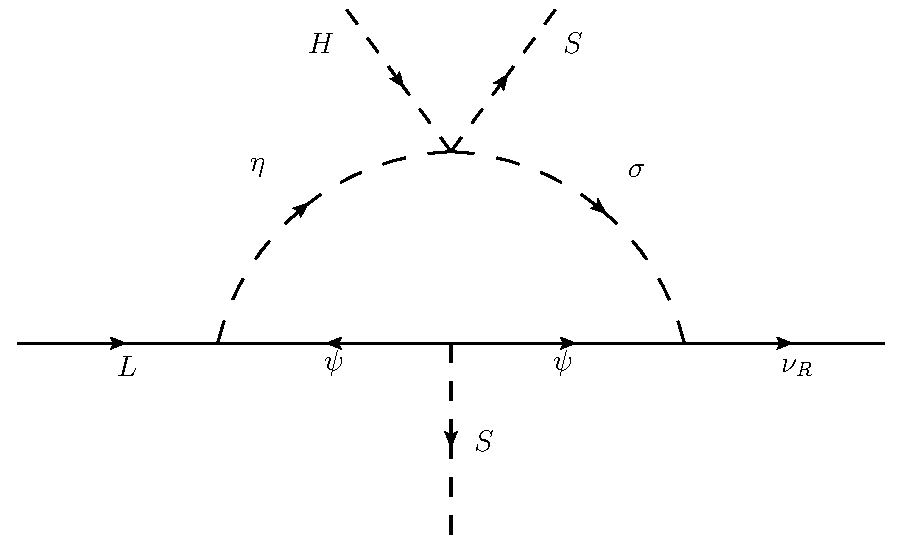
\includegraphics[scale=0.75]{Neutrino_Loop.pdf}
\caption{One-loop generation of Dirac neutrino mass}
\label{fig:zee}
\end{figure}
%
 The Dirac neutrino mass matrix in this model is generated at one loop-level according to the diagram in  fig.~\ref{fig:zee}. The expression for $\mathcal{M}_{\nu}$ is given by~\cite{Reig:2018mdk}
%
\begin{align}
(\mathcal{M}_{\nu})_{ij} = \frac{\lambda_8 v_S v}{32 \pi^{2}} \sum_{a=1}^{3} \frac{h_{i a} M_{\psi_{a}}y^{\dagger}_{a j}} {m_{\chi_{R_2}}^{2}-m_{\chi_{R_1}}^{2}} \left[ F\left( \frac{m_{\chi_{R_2}}^{2}}{M_{\psi_{a}}^{2}} \right) - F\left( \frac{m_{\chi_{R_1}}^{2}}{M_{\psi_{a}}^{2}} \right) \right] + (R \to I)\,,
\end{align}
%
%check the following formula:
where $F(x) =x \log x/(x-1)$ is the loop function, $M_{\psi_{a}}$ is
the fermion mass and $\chi_{R_{(1,2)}}$ ( $\chi_{I_{(1,2)}}$ ) are the
two CP-even (CP-odd) mass eigenstates.
To obtain neutrino masses it is necessary that $\mu \neq 0$. In this
way, in addition to the suppression from the seesaw mechanism, we can
have further suppression in the neutrino mass matrix for small values
of $\mu$.
The structure of the effective neutrino mass matrix is given by the
product $(M_{\nu})_{ij} \propto h_{i a} y_{a j}$, which is similar to
the structure of the neutrino mass matrix for the tree-level seesaw
mechanism for Dirac neutrinos~\cite{Chulia:2016ngi}. 

If only one
fermion $\psi_R$ is added, we will have two massless neutrinos, which
does not agree with the current data obtained from the neutrino
experiments~\cite{deSalas:2017kay}. In our case, we will assume the
existence of three fermions, generating Dirac scotogenic masses for
the two neutrinos ($\nu_{k}$ is massless due to the assignment of
charges). If we consider the case in which $m_{\eta^{\pm}}^2 = \mu_{\sigma} \gg \frac{1}{2} \lambda_8 v v_S$ and $\lambda_7$, $\lambda_2$, $\lambda_4 \gg 1$. Taking $m_{\chi_{R_{2}}}-m_{\chi_{R_{1}}} = \lambda_8 v v_{S}$ and $m_{\chi_{R_{2}}}+m_{\chi_{R_{1}}} = 2 m_{\eta^{\pm}}^{2}$ one finds
%
\begin{align*}
(\mathcal{M}_{\nu})_{ij} = \frac{\lambda_8 v_S v}{16 \pi^{2}} \sum_{a=1}^{3} \frac{h_{i a} M_{\psi_{a}}y^{\dagger}_{a j}} {m_{\eta^{\pm}}^{2}-M_{\psi_{a}}^{2}} \left[1 - \frac{M_{\psi_{a}}^{2}}{m_{\eta^{\pm}}^{2}-M_{\psi_{a}}^{2}} \log \left( \frac{m_{\eta^{\pm}}^{2}}{M_{\psi_{a}}^{2}} \right)\right]\,,
\end{align*}
%
and if we take $m_{\eta^{\pm}}^{2} \gg M_{\psi_{a}}^{2}$ one has 
%
\begin{align}
(\mathcal{M}_{\nu})_{ij} & = \frac{\lambda_8 v_S v}{16 \pi^{2}} \sum_{a=1}^{3} \frac{h_{i a} M_{\psi_{a}}y^{\dagger}_{a j}} {m_{\eta^{\pm}}^{2}}\,, \\
& \sim 0.006~\text{eV} \left( \frac{\lambda_8}{1 \text{GeV}}\right) \left( \frac{v_{S}}{10 \text{TeV}}\right) \left( \frac{M_{\psi_{a}}}{1 \text{TeV}}\right) \left( \frac{50 \text{TeV}}{m_{\eta^{\pm}}}\right)^{2} \left( \frac{h_{i a} y_{a j}^{\dagger}}{10^{-6}}\right)\,. \nonumber
\end{align}
%
The mass matrix for Dirac neutrinos is diagonalized by
\begin{align*}
(U^{\nu}_R)^{\dagger} \mathcal{M}_{\nu} U^{\nu}_L = \mathcal{M}_{\nu}^{\text{diag}} = \text{diag}(m_1, m_2, m_3)\,,
\end{align*}
where $U^{(\nu)}_R$ and $U^{(\nu)}_L$ are unitary $3 \times 3$
matrices. The leptonic charged currents with non-massless neutrinos
are parametrized in terms of the unitary mass
\begin{align*}
U_{\text{PMNS}} = \left( U^{\ell}_L \right)^{\dagger} U^{\nu}_L\,,
\end{align*}
where is the left diagonalization matrix of the charged leptons.
As we already are in the diagonal basis after the calculation of the
one-loop neutrino masses, we can set
$U_{L}^{\ell} = \mathds{1}$. Moreover, we assume that $U_{R}^{\nu} = \mathds{1}$.
Therefore, we can express the Dirac neutrino mass matrix in the
following way
\begin{align}
(\mathcal{M}_{\nu})_{ij} = (U_{\text{PMNS}})_{ij} (\mathcal{M}_{\nu}^{\text{diag}})_{j}\,,
\end{align}
where the matrix $U_{\text{PMNS}}$ is expressed in the standard parameterization as
\begin{align*}
U_{\text{PMNS}} = \begin{pmatrix}
    1 & 0		& 0 \\
    0 & c_{23}  & s_{23} \\
    0 & -s_{23} & c_{23}
\end{pmatrix}
\begin{pmatrix}
    c_{13}  &  0 & s_{13}e^{-i\delta} \\
    0 		&  1 & 0 \\
    -s_{13}e^{i\delta} &  0 & c_{13}
\end{pmatrix}
\begin{pmatrix}
    c_{12}  & s_{12} & 0 \\
    -s_{12} & c_{12} & 0 \\
    0		& 0		 & 1
\end{pmatrix}\,,
\end{align*}
where $s_{ij} = \sin \theta_{ij}$ and $c_{ij} = \cos \theta_{ij}$ and $\theta_{ij}$ are neutrino mixing angles and $\delta$ is CP-violating phase.

\section{Lepton flavor violation}
\label{sec:LFV}
%
\begin{figure}
\centering
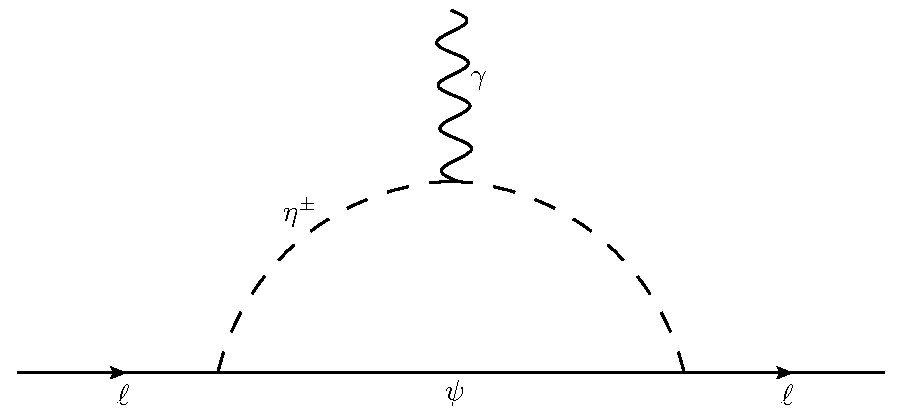
\includegraphics[scale=0.6]{LFV.pdf}
\caption{Feynman diagram for process $l^{-}_{i} \to l^{-}_{j} \gamma$}
\label{fig:LFV}
\end{figure}
%
The new Yukawa interactions in eq.~\eqref{eq:LagY} in our model introduce processes of charged lepton flavor violation (CLFV). These CLFV processes are induced at one loop level, as shown in the fig.~\ref{fig:LFV}. In this case, the $\overline{L} \tilde{\eta} \psi_R$ interaction allows the part of the double scalar $\eta$ ($\eta^{\pm}$) to mediate in the loop.

The most common search for CLFV focuses on the $l^{-}_{i} \to l^{-}_{j} \gamma$ process. This process is described by the effective Lagrangian
%
\begin{align}
    \mathcal{L} = \frac{\mu_{m}^{\alpha \beta}}{2} l^{-}_{\beta} \sigma^{\mu \nu} l^{-}_{\alpha} F_{\mu \nu}
\end{align}
%
where $\mu_{m}^{\alpha \beta}$ is a transition magnetic moment~\cite{Toma:2013zsa}.
The decay rate is given by~\cite{Lavoura:2003xp}
%
\begin{align}
 \Gamma(l^{-}_{i} \to l^{-}_{j} \gamma) = \frac{m^{3}_{i}}{16 \pi} \left| \sum_{\alpha} h^{\alpha}_{i} m_{i} h^{\alpha}_{j} \frac{i e}{16 \pi M^{2}_{\eta^{-}}} K(t_{k}) \right|^{2}\,, 
\end{align}
%
where $t_{\alpha} = M^{2}_{\psi_{\alpha}}/M^{2}_{\eta^{-}}$ and
%
\begin{align}
    K(t_{\alpha}) = \frac{2t_{\alpha}^{2}+5t_{\alpha}-1}{12(t_{\alpha}-1)^{3}} - \frac{t_{\alpha}^{2}\log t_{\alpha}}{2(t_{\alpha}-1)^{4}}\,.
\end{align}
%
If we assume that $t_{\alpha} \to 0$, $t_{\alpha} \to 1$ and $t_{\alpha} \to \infty$, we have that $K(t_{\alpha}) = 1/12$, $K(t_{\alpha}) = 1/24$ and $K(t_{\alpha}) = 1/(6t)$, respectively.

For $i \neq j$ we have CLFV processes, these processes are severely restricted by the current bounds , which set limits to the Yukawas. The most restrictive experimental bounds is decay $\mu \to e \gamma$, which is several orders of magnitude greater than radiative decays $\tau \to~l\gamma$, with $l = e, \mu$. These restrictions are given by Br$(\mu \to e\gamma)$ \textless $5.7 \times 10^{-13} $~\cite{Adam:2013mnn}, Br$(\tau \to e\gamma) $\textless$ 3.3 \times 10^{-8}$ and Br$(\tau \to~\mu\gamma) $\textless$ 4.4 \times 10^{-8}$~\cite{Aubert:2009ag, Bona:2007qt, Miyazaki:2012mx}. 

In the limit $m_{\eta^{\pm}}^{2} \gg M_{\psi_{a}}^{2}$, $t_{\alpha} \to 0$ the decay width reads
%
\begin{align}
 \Gamma(l^{-}_{i} \to l^{-}_{j} \gamma) = \frac{m^{3}_{i}}{16 \pi} \left| \sum_{\alpha} h^{\alpha}_{i} m_{i} h^{\alpha}_{j} \frac{i e}{16 \pi M^{2}_{\eta^{-}}} \left[ \frac{1}{12} \right] \right|^{2}\,, 
\end{align}
%
using the current experimental constraint, can be fullfilled provided
%
\begin{align*}
    \left( \sum_{\alpha} \frac{h^{}_{i \alpha} h_{\alpha j}^{*}}{M^{2}_{\eta^{-}}} \right)^{2} \leq 5.7 \times 10^{-13} \frac{768 \pi G_{F}^{2}}{\alpha_{EM}}
\end{align*}
%
which leads to a very slight requirement,
\begin{align*}
    \left| \sum_{\alpha}h^{}_{i \alpha} h_{\alpha j}^{*}\left(\frac{50\text{TeV}}{M^{2}_{\eta^{-}}} \right)^{2} \right| \leq 12.65
\end{align*}
%
For $i = j$ we have processes that contribute to the leptonic magnetic dipole moment. In the case of the anomalous muon magnetic dipole moment, the experimental measurements does not agree with the values predicted by the SM~\cite{Lindner:2016bgg}. This can be a proof of the veracity of the model, in addition to giving restrictions on the Yukawas.

\section{Dark matter}
\label{sec:DM}
From table~\ref{tab:partcont}. we can see that after the spontaneous breaking of
$\operatorname{U}(1)_X$ there is remnant $Z_2$ symmetry under which the particles circulating the loop in fig.~\ref{fig:zee}. plus $\nu_{R3}$ are odd, while the other right handed neutrinos and the SM particles are even. The lightest odd particle can be a dark matter candidate. In this way we can have either fermionic or scalar dark matter in the model.

\subsection{Fermionic dark matter}
The relic density of DM is controlled by the $Z'$ portal~\footnote{For
  a recent review of Majorana Dark matter with a $Z'$ portal
  see~\cite{Blanco:2019hah} } and
% check Ibarra papers
also through the annihilation
$\psi_{1} \psi_{1} \to l _{\alpha}^+ \overline{l}_{\beta}^- $, via
Yukawa coupling $h^{a}_{i}$. These Yukawa couplings are restricted by
CLFV and neutrino masses. %But, Yukawa couplings $y^{a}_{j}$ is free.
In the case where the mass of the other fermions and scalars is nearly
degenerated to $\psi_{1} $, the processes of coannihilation can be
relevant for the relic density calculation~\cite{Klasen:2013jpa}.

Because the particle $\psi_{1}$ only interacts with the leptons via the Yukawa couplings, this model has no a direct detection cross section at three level. 

% In the case that the mass of the lightest fermion $\psi$ is smaller
% than the mass of the scalars, the DM will be fermionic. For this DM it
% is possible to have the following observable decay of the scalar
% $\eta^{\pm} \to l^{\pm} \psi_{1}$, therefore, the other fermions decay
% as $ \psi \to l^{\pm} l^{\mp} \psi_{1}$ and
% $\psi \to l^{\pm} l^{\mp} \psi_{1,2} $, through $\eta^{\pm}$.

\subsection{Scalar dark matter}
Contrary to fermionic DM, scalar DM has additional interactions beyond the Yukawa couplings  which can be used to control relic density. This corresponds to the simplified dark matter model of scalar singlet-doblet dark matter, which have been studied in detail in~\cite{} 

When the lightest scalar  is mainly a scalar doublet, the phenomenology will be similar inert doublet model~\cite{Honorez:2010re}. For this kind of DM model  inert doublet model there are two mass regions for DM which can to reproduce adequately the relic density ($50$GeV \textless $m_{DM}$ \textless $70$GeV and $535$GeV \textless $m_{DM}$ \textless $20$TeV)~\cite{Garcia-Cely:2015khw}.

% In recent studies, these two regions are connected through use of a
% second doublet~\cite{Borah:2019aeq}. How we have in the model the
% Yukawa coupling, the decay $\psi_{i} \to l^{\pm} \eta^{\mp}$ is
% possible. In addition, decay is given via scalar interactions
% $\eta^{\pm} \to \eta^{0} + {W^{\pm}}$, where $W^{\pm}$ can be real or
% virtual and decay to leptons or quarks.

Now, if the lightest scalar is mainly a singlet, the DM will be
similar to Singlet Scalar Dark Matter
Model~\cite{Athron:2017kgt}\todo{change for the original ref by Ma et
  al. etc}.
The mass range for the scalar singlet that produces the adequate relic
density is around the Higgs resonance and for masses above $1$TeV. For
this model~\cite{}, the relevant coupling for DM phenomenology is the
Higgs portal trough the Lagrangian term $\sigma^{2} H^{2}_{i}$.
This term generates interesting phenomenological consequences.
Such as, thermal production of DM in the early
universe~\cite{Yaguna:2008hd}, direct detection and invisible decay of
SM Higgs through $h \to \sigma \sigma$~\cite{Mambrini:2011ik}.
In addition, this model has important contributions for cosmology, in
phenomena such as inflation~\cite{Lerner:2009xg} and
baryogenesis~\cite{Cline:2012hg}.

\section{Cosmological constraints}

A not-so-minimal model can be obtained as the one-loop realization of
the effective 5-dimensional operator for Dirac neutrino masses~\cite{Gu:2006dc}
\begin{align}
  \label{eq:ld5}
  \mathcal{L}_{5D}=\frac{1}{\Lambda} \overline{L_i} H \nu_R S\,,
\end{align}
as displayed in fig.~\ref{fig:ld5}.
In this case we can use the standard $\operatorname{U}(1)_{B-L}$
charge of $-1$ for the lepton doublets.
It is well established that the solution for anomaly cancellation
conditions with three quiral fields with exotic
$\operatorname{U}(1)_{B-L}$ charges: $-4$,~$-4$,~$5$,  when assigned to the
three light right-handed neutrinos can forbid three level Dirac and
Majorana masses~\cite{Calle:2018ovc}.
The presence of a set of heavy Majorana mediators to realize the
dimension-5 operator at one-loop with the diagram in
fig.~\ref{fig:ld5}., would spoil the anomaly cancellation conditions.
However, we can further add an extra set of quiral fermion in a
vector-like way, such that the full set heavy fermions do not affect
the anomaly cancellation. A such assignment is displayed in
Table~\ref{tab:partcont2}.
The fields $\xi_{L \alpha}$ guarantee the anomaly cancellation and
their Majorana masses are obtained in the same way than the ones for
$\psi_{R\alpha}$.


\begin{figure}
\centering
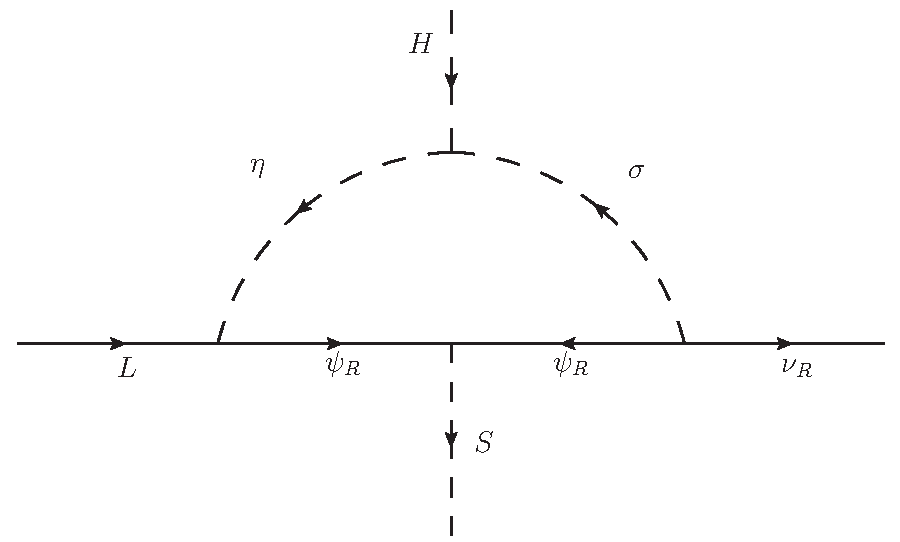
\includegraphics[scale=0.75]{Neutrino2.pdf}
\caption{One-loop realization of the dimension-5 effective Dirac neutrino mass operator }
\label{fig:ld5}
\end{figure}
%

\begin{table}
  \centering
  \begin{tabular}{|c|c|c|c|c|c|c|c|}
    \hline  
    Fields     & $\operatorname{SU}(2)_L$ & $\operatorname{U}(1)_Y $ & $\operatorname{U}(1)_{B-L}$& $\operatorname{U}(1)_A$& $\operatorname{U}(1)_B$& $\operatorname{U}(1)_D$& $\operatorname{U}(1)_G$\\ \hline
$d_R $  & $\boldsymbol{1}$& $-1/2$  &  $1/3$&  $-1$&  $1$&  $0$&  $2/3$ \\
$u_R $  & $\boldsymbol{1}$& $+2/3$  &  $1/3$&  $1$&  $-1$&  $1$&  $-1/3$ \\
$Q $  & $\boldsymbol{2}$& $-1/6$  &  $1/3$&  $0$ &  $0$&  $1/2$&  $1/6$ \\\hline
$e_R $  & $\boldsymbol{1}$& $-1$  &  $-1$&  $1$ &  $-1$ &  $-2$&  $0$ \\
$L $  & $\boldsymbol{2}$& $-1/2$  &  $-1$&  $0$ &  $0$ &  $-3/2$&  $-1/2$ \\
$H $  & $\boldsymbol{2}$& $-1/2$  &  $0$&  $1$ &  $-1$ &  $1/2$&  $-1/2$ \\
$\eta$  & $\boldsymbol{2}$ & $+1/2$  & $5/2$& $-3/2$ &$3/2$ &$3$&$2$ \\
$S$ & $\boldsymbol{1}$ & $0$  & $3$& $-3$ & $3$ & $3$& $3$ \\
$\sigma$ & $\boldsymbol{1}$ & $0$ & $5/2$& $-5/2$ & $5/2$ & $5/2$& $5/2$ \\
\hline
 $\nu_{Ri}$ & $\boldsymbol{1}$ & $0$ & $-4$& $4$ & $-4$ & $-4$& $-4$\\
$\nu_{R3}$ & $\boldsymbol{1}$ & $0$ & $+5$& $-5$ & $5$ & $5$& $5$\\
$\psi_{R\alpha}$  & $\boldsymbol{1}$ & $0$ & $3/2$& $-3/2$ & $3/2$ & $3/2$& $3/2$ \\\hline
$\xi_{L\alpha}$  & $\boldsymbol{1}$ & $0$ & $3/2$ & $-3/2$ & $3/2$ & $3/2$& $3/2$\\\hline
  \end{tabular}
  \caption{The new scalars and fermions with their respective charges. The SM fields have the usual $U(1)_{B-L}$ assignment. Now $\alpha=1,2$}
    \label{tab:partcont2}
\end{table}

In this way we end up with a model with four Majorana fermions, one more than in the minimal solution. Alternatively we can have a single set of $\psi_R$ and $\xi_L$ but with two set of scalars $\eta_\alpha$, $\sigma_{\alpha}$~\cite{Reig:2018mdk}. If we choose $r$ as a fraction with denominator $2$, let say $r=3/2$, the $\operatorname{U}(1)_{B-L}$ left out a remnant $Z_2$ discrete symmetry which guarantees the stability of the lightest odd-particle.

The two additional left-handed fields $\xi_{L\alpha}$,  with a $\operatorname{U}(1)_{B-L}$ charge of $r=3/2$,  cancel out the anomalies. Moreover, we have both Dirac mass terms $\overline{\xi_{L \alpha}}\psi_{R \beta}$ and $ \overline{\xi_{L\alpha}^c }\xi_{L \beta} \langle S\rangle$ and the full set of Majorana fields are massive and heavy. The lighter of them a would be dark matter candidate.

% \footnote{Check 2r+2nu: -2,6,7,-9,-3  3r+2nu: -(5/2),7/2,-7,6,9/2}

The coupling of $Z'$ with the lepton doublets opens up the possibility
of thermalization of the right handed neutrinos in the primordial
plasma.
In fact, the existence of three new right neutrinos in nature
contribute to the total energy density of the universe. These new
contributions can modify the cosmological observables in the cosmic
microwave background (CMB). These new neutrinos contribute to the
existence of dark radiation, which affects the expansion processes of
the universe and the number of relativistic degrees of freedom for
neutrinos.

In the case of our model, the new gauge symmetry introduces  new gauge boson that mediates interaction of the right neutrinos and the SM. This allows the right neutrinos to thermally modify the relativistic degrees of freedom with contributions given by~\cite{Anchordoqui:2012qu,Anchordoqui:2011nh}
%
\begin{align*}
    \Delta N_{\text{eff}} = N_{\text{eff}} - N^{\text{SM}}_{\text{eff}} = N_{\nu_R} \left( \frac{T_{\nu_{R}}}{T_{\nu_{L}}} \right)^{4} = N_{\nu_R} \left( \frac{g(T^{\nu_{L}}_{\text{dec}})}{g(T^{\nu_{R}}_{\text{dec}})} \right)^{4}
\end{align*}
%
where $ g(T) $ is the number of relativistic degrees of freedom at a temperature $T$ in the SM~\cite{Aghanim:2018eyx}. The decoupling temperature of the left neutrinos $\nu_L$ is $ T^{\nu_{L}}_{\text{dec}} \approx 2.3 $ MeV~\cite{Enqvist:1991gx}, when $g(T^{\nu_{L}}_{ \text{dec}}) = 43/4 $ corresponding to the three $\nu_{L}$, $e^{\pm} $ and the photon~\cite{Kolb:1990vq}. The rate of interaction of the right neutrinos with the SM is mediated by the gauge boson $Z^{\prime} $ and is given by~\cite{SolagurenBeascoa:2012cz}
%
\begin{align*}
    \Gamma_{\nu_R} (T) &= n_{\nu_R}(T) \langle \sigma(\overline{\nu_{R}} \nu_{R} \to \overline{f} f) \upsilon \rangle \,, \\
    &= \frac{g^{2}_{\nu_R}}{n_{\nu_R}(T)} \int \frac{d^{3} p}{(2 \pi)^{3}} f_{\nu_R}(p) \int \frac{d^{3} k}{(2 \pi)^{3}} f_{\nu_R}(k) \sigma_{f}(s) \upsilon\,,
\end{align*}
%
where $f_{\nu_R}(k)=1/(e^{k/T}+1)$ is the Fermi-Dirac distribution, $g_{\nu_R} = 2$ is the spin number, $\upsilon = 1-\cos{\theta}$ is the Moller velocity, $s = 2 p k (1-\cos{\theta})$, where $p$ and $k$ are the momenta of the particle and $\theta$, the angle between them, and the number density of right-handed neutrinos is given by
\begin{align*}
n_{\nu_R}(T) = g_{\nu_R} \int \frac{d^{3} k}{(2 \pi)^{3}} f_{\nu_R}(k)\,.
\end{align*}

The cross section is given in~\cite{Barger:2003zh}, in the case with heavy mediator $T^{\nu_R}_{\text{dec}} \ll M_{Z^{\prime}}$, we can to take the limit when $s \ll M_{Z^{\prime}}$ and neglecting the fermion masses, we have that the cross section is
%
\begin{align*}
    \sigma_{f}(s) \approx N^{C}_{f} \frac{s}{12 \pi} \left( \frac{g^{\prime}}{M_{Z^{\prime}}} \right)^{4} Q^{2}_{\nu_R} (Q^{2}_{f_L} + Q^{2}_{f_R})\,,
\end{align*}
%
where $N^{C}_{f}$ is the color multiplicity of the fermion, i.e. $N^{C}_{q(\ell)} = 3(1)$, $Q_{f}$ is the charge of the fermion under the new symmetry, $g^{\prime}$ and $M_{Z^{\prime}}$ are the gauge coupling and mass for the new gauge boson. Solving the integrals with this last cross section we obtain that the interaction rate is given by
%
\begin{align*}
    \Gamma_{\nu_{R}}(T) = \frac{49 \pi^{5} T^{5}}{97200 \zeta(3)} \left( \frac{g^{\prime}}{M_{Z^{\prime}}} \right)^{4} \sum_{f} N^{C}_{f} Q^{2}_{f}\,,
\end{align*}
%
where the sum is performed over all SM fermion that are in thermal equilibrium with the plasma at temperature $T$. To estimate the contribution to the relativistic degrees of freedom for neutrinos, it is necessary to calculate the decoupling temperature of the right neutrinos ($T^{\nu_R}_{\text{dec}}$). The latter occurs when the interaction rate of neutrinos with the SM drop below the rate of expansion of the universe, i.e.
%
\begin{align*}
\Gamma(T^{\nu_R}_{\text{dec}}) = H(T^{\nu_R}_{\text{dec}})\,, 
\end{align*}
%
where the Hubble expansion parameter is
%
\begin{align*}
    H(T) = \sqrt{\frac{8 \pi G_{N} \rho(T)}{3}} = \sqrt{\frac{4 \pi^{3} G_{N}}{45} \left( g(T) + \frac{21}{4} \right)} T^{2}\,,
\end{align*}
%
and the $21/4$ correspond to the contribution of the right neutrinos to relativistic degrees of freedom. By finding the decoupling temperature of the right neutrinos $T^{\nu_R}_{\text{dec}} $ by a root finding method, it is possible to calculate $\Delta N_{\text{eff}}$.

The results of $T^{\nu_R}_{\text{dec}}$ and $\Delta N_{\text{eff}}$ as a function of $M_{Z^{\prime}}/g^{\prime}$ are exhibited in fig.~\ref{fig:Neff}. We can see that for small decoupling temperatures, the variation in the number of relativistic degrees of freedom of the new species is large and vice versa. The bound that come from Planck~\cite{ghanim:2018eyx} is stronger than the bound of LEP~\cite{Alioli:2017nzr}. For our model we find that $M_{Z^{\prime}}/g^{\prime} \gtrsim 60$TeV in order to satisfy the conditions of $N_{eff}$.



%
\begin{figure}
\centering
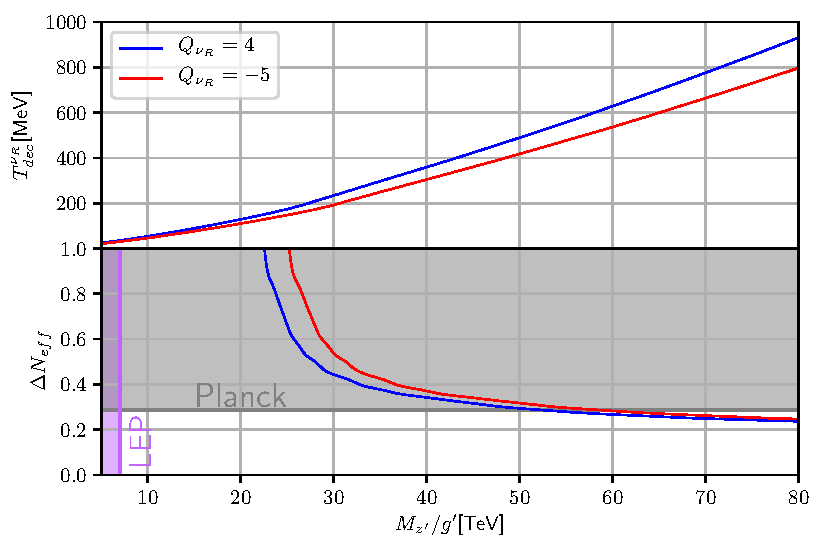
\includegraphics[scale=0.8]{DeltaNeff.pdf}
\caption{In the upper panel is the decoupling temperature of the right neutrino $\nu_{R}$ in function of $M_{z^{\prime}}/g^{\prime}$. In the lower panel is the additional contribution to the number of relativistic degrees of freedom ($\Delta N_{\text{eff}}$) in function of $M_{z^{\prime}}/g^{\prime}$. The gray shaded region is excluded by the measurements in the Planck CMB~\cite{Aghanim:2018eyx}. The region shaded in violet shows the bound from LEP  LEP~\cite{Alioli:2017nzr}.}
\label{fig:Neff}
\end{figure}
%




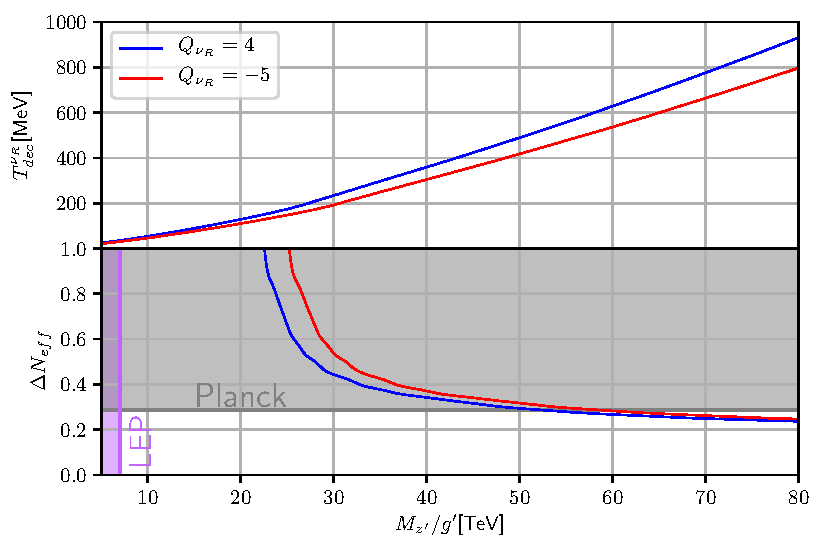
\includegraphics[scale=0.9]{DeltaNeff.pdf}


\appendix

\section{General solution}

The general solution to fig.~\ref{fig:zee} is
\begin{align}
  L=&\nu_R+4\psi_R -H \,,& \eta=& H-\nu_R-3\psi_R \nonumber\\
  \sigma=& -\nu_R-\psi_R\,,&S=& 2\psi_R \,.
\end{align}
The consistency condition for $H=0$ is
\begin{align}
  L=\nu_R+4\psi_R\,.
\end{align}

On the other hand, for fig.~\ref{fig:ld5}
\begin{align}
  L=&-H+\nu_R+2\psi_R &
  \eta=&H-\nu_R-\psi_R \nonumber\\
  \sigma=& -\nu_R-\psi_R\,,&S=& 2\psi_R \,.
\end{align}
$\nu_R$, $H$  and $L$ are fixed from the anomaly cancellation conditions.


%\bibliographystyle{h-physrev4}
%\bibliographystyle{JHEP-2}
%\bibliographystyle{JHEP}
\bibliographystyle{apsrev4-1long}
%\bibliographystyle{apsrev4-1longdoi}
\bibliography{susy}



\end{document}

%%% Local Variables: 
%%% mode: latex
%%% TeX-master: "draft"
%%% ispell-local-dictionary: "american"
%%% End: 
